%%%%%%%%%%%%%%%%%%%%%%%%%%%%%%%%%%%%%%%%%%%%%%%%%%%%%%%%%%%%%%%%%%%%%%
% DelaunayTriangulationSpannerNotes
% March 20th, 2013
% By Simon Pratt (mostly)
\documentclass{tufte-handout}

\usepackage{CGAlgorithms}
\usepackage{QuestionAnswer}
\usepackage{TheoremStuff}
\usepackage{HeaderStuff}
\usepackage{natbib}
\usepackage[pdftex]{graphicx}

%%%%%%%%%%%%%%%%%%%%%%%%%%%%%%%%%%%%%%%%%%%%%%%%%%%%%%%%%%%%%%%%%%%%%%
% Configuration
\newcommand{\DocTitle}{Delaunay Triangulation Spanner Notes}
\newcommand{\DocAuthor}{Simon Pratt}

\title{\DocTitle}
\author{\DocAuthor}
\fancyhead[L]{\DocTitle}
\fancyhead[R]{\DocAuthor}
\bibliographystyle{plain}

%%%%%%%%%%%%%%%%%%%%%%%%%%%%%%%%%%%%%%%%%%%%%%%%%%%%%%%%%%%%%%%%%%%%%%
% Document
\begin{document}

\maketitle

% Content starts here

\part{Dobkin's Results}

The Delaunay triangulation of a set of points in the plane is a
spanner with spanning ratio $c \le ((1 + \sqrt{5})/2)\pi \approx
5.08$.  This was proven in the paper ``Delaunay Graphs Are Almost as
Good as Complete Graphs'' by Dobkin, Friedman, and Supowit
\cite{Dobkin:1987} \cite{Dobkin:1990}.

\section{Introduction}

Let $S$ be a set of points in the plane and $DT(S)$ be the edges of
the Delaunay triangulation of $S$.

We consider the path between two arbitray points $a,b \in S$.  Let the
line connecting $a,b$ be the \emph{direct line}.  We construct
\emph{the direct DT path} by walking along the direct line, each time
a new face of the Voronoi diagram is reache we add the corresponding
Delaunay edge.

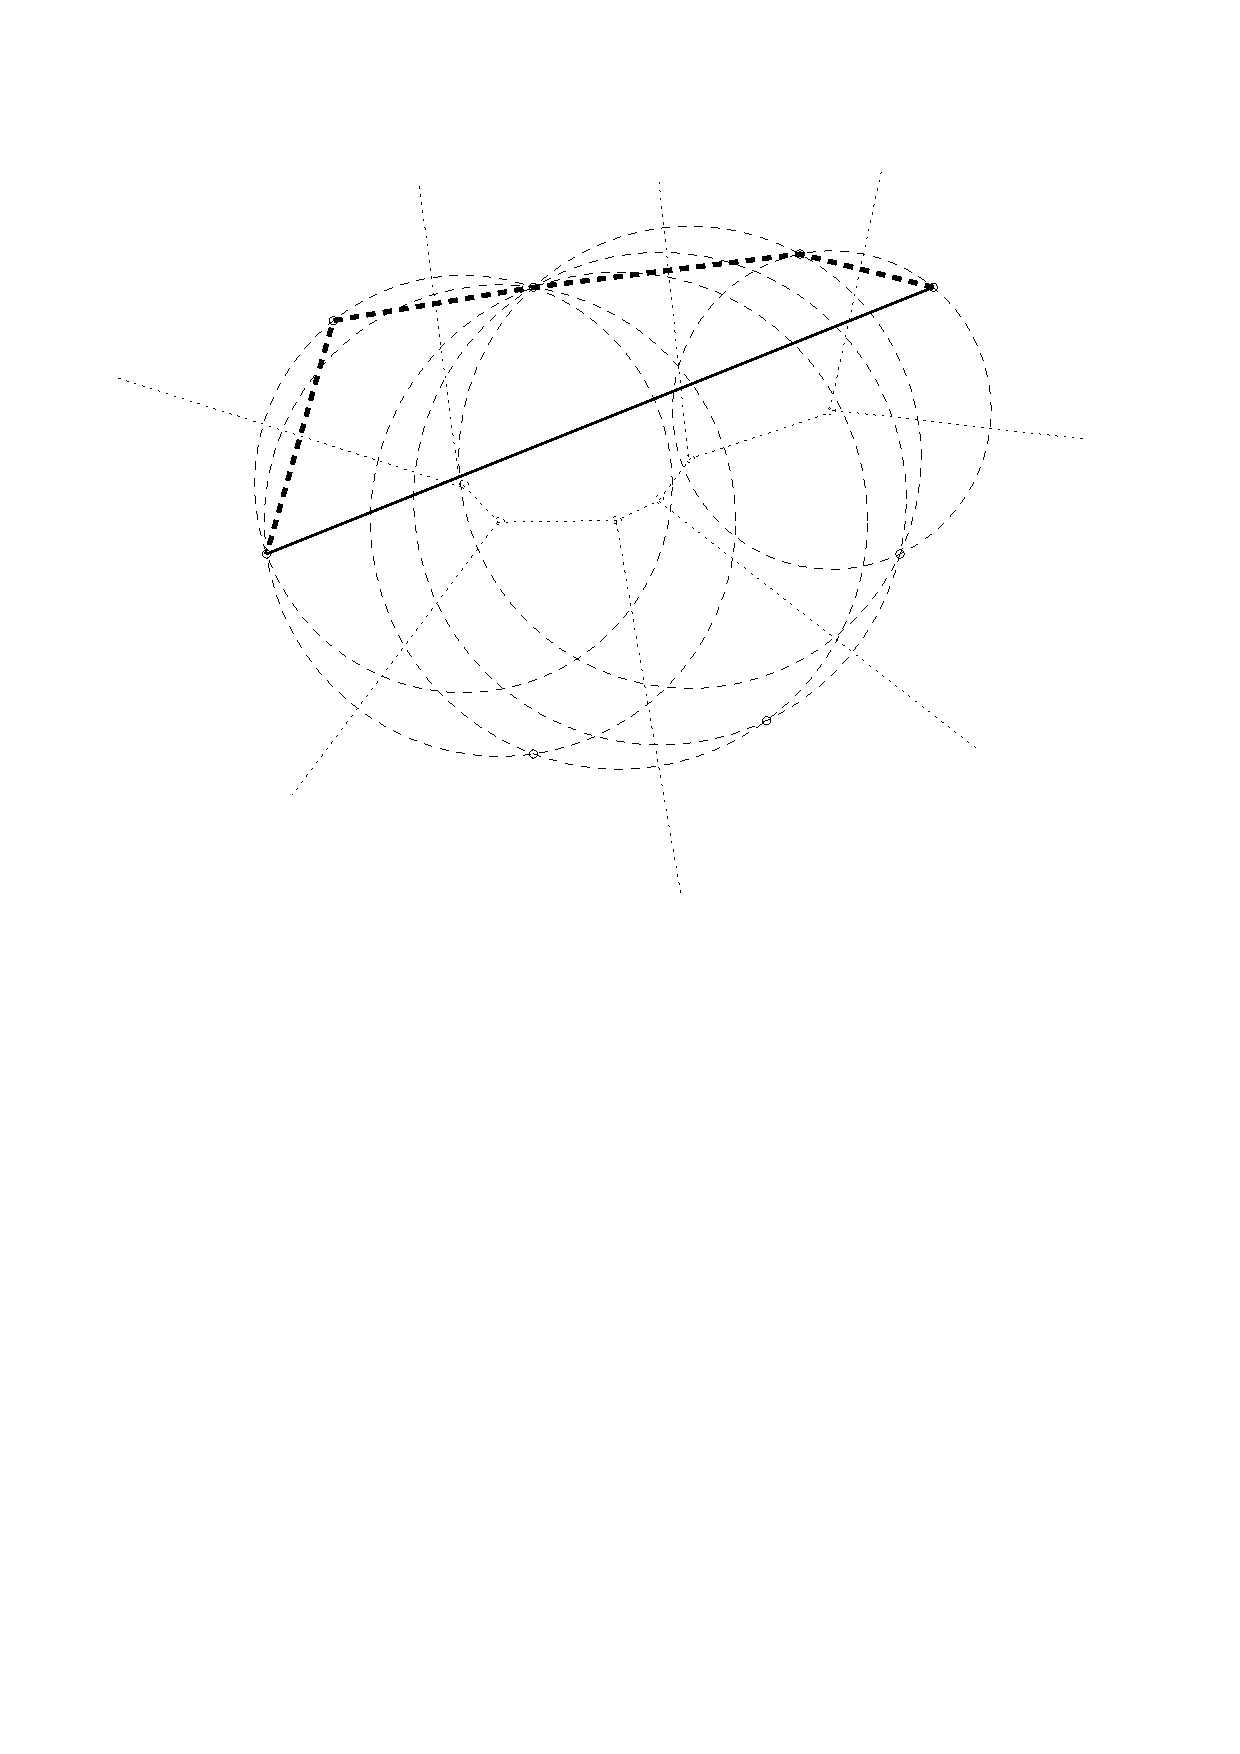
\includegraphics[scale=0.75]{figures/voronoi2.pdf}

\section{One-Sided Path: The Easy Case}

If all edges along the direct DT path between points $a,b \in S$ are
either all above or all below the direct line, we say that this is a
one-sided path.

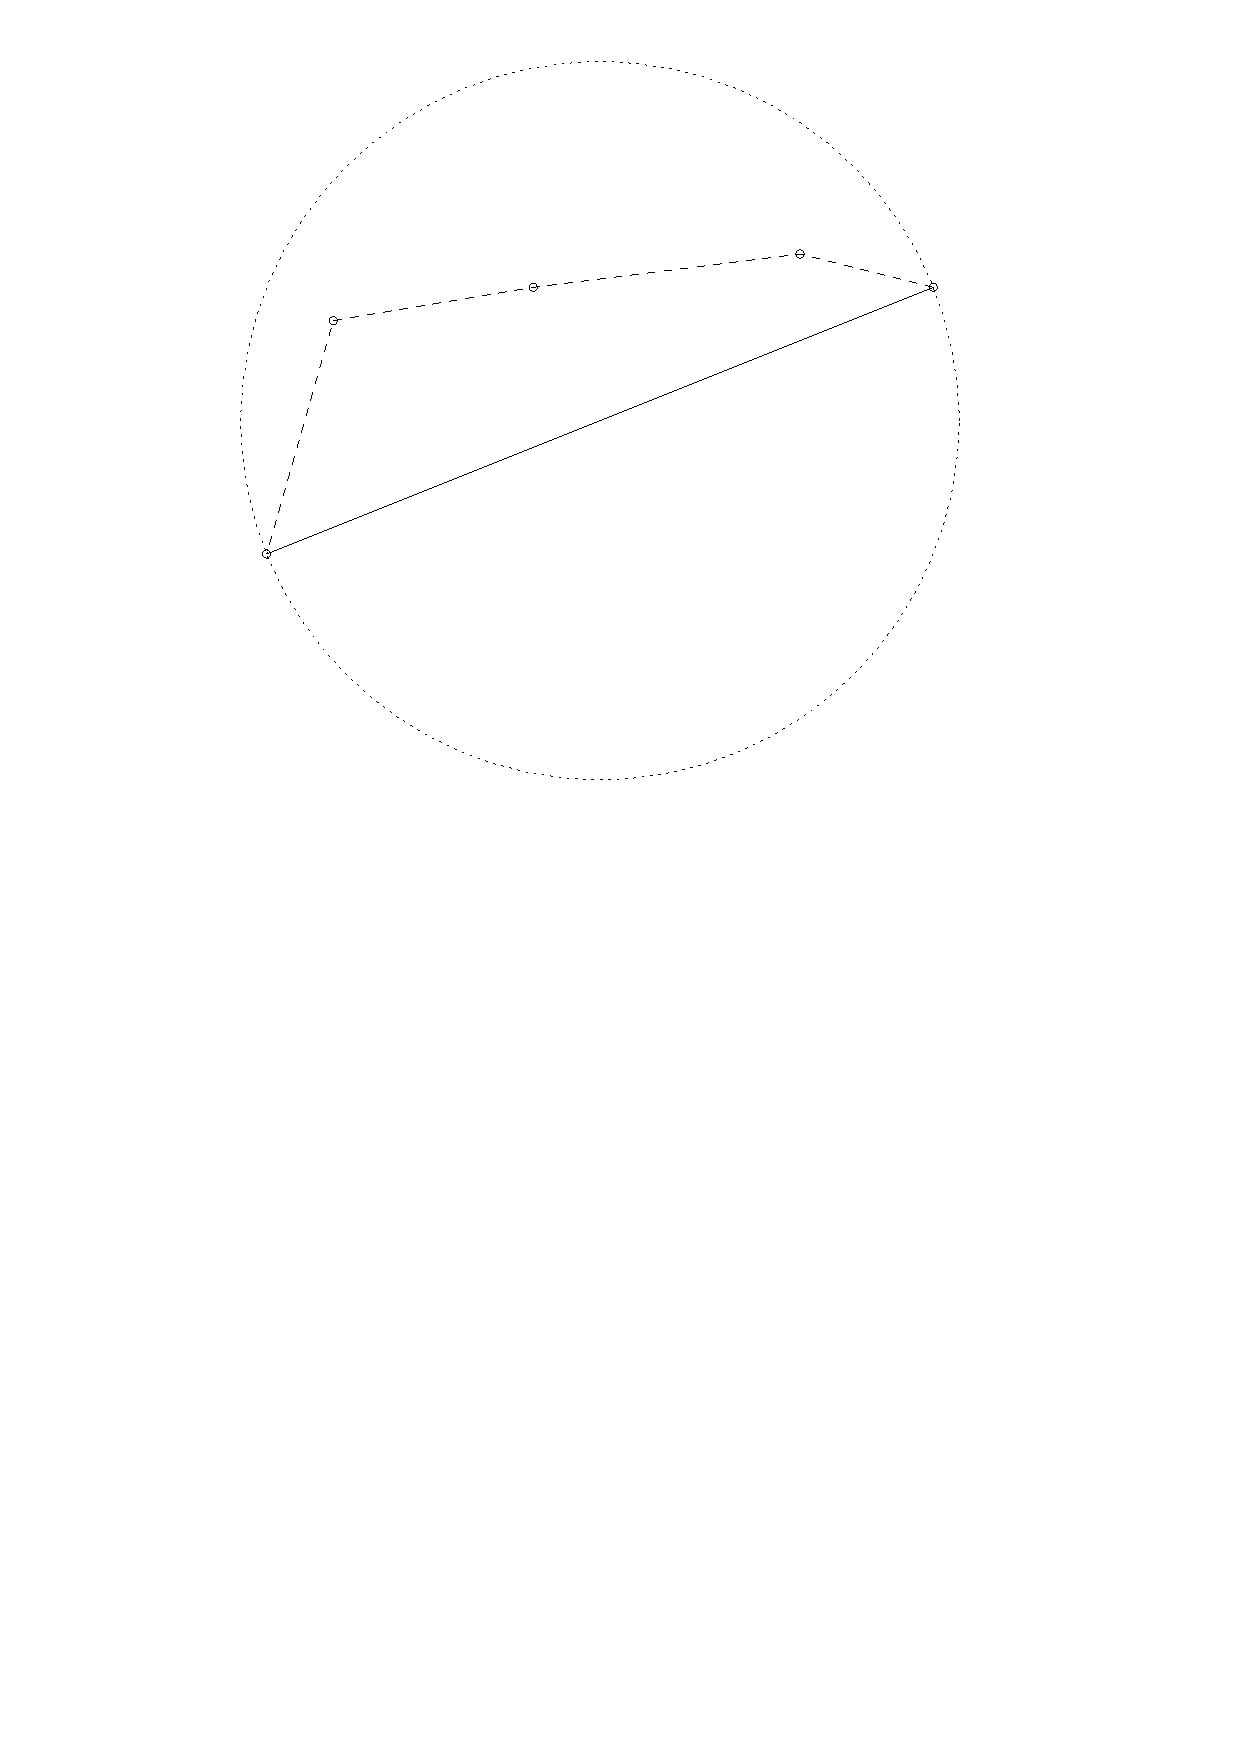
\includegraphics[scale=0.75]{figures/one-sided_path.pdf}

\begin{Lemma}

  Points along a direct DT path are monotonic in $x$.

\end{Lemma}

\begin{Lemma}

  All points along the direct DT path from $a$ to $b$ are contained
  within or on the boundary of the circle with $a$ and $b$
  diametrically opposed.
  
\end{Lemma}

\begin{Lemma}

  The boundary of a connected union of circles has boundary at most
  $\pi \cdot (x_r - x_l)$ where $x_r$ and $x_l$ are the extreme x
  coordinates of any of the circles.
  
\end{Lemma}

From these lemmas, it follows that the one-sided path is at most
$\pi/2$ times as long as the euclidean distance between the endpoints.

\section{The Harder Case}

The direct DT path may cross the direct line $\BigOmega{n}$ times,
which can yield a much longer path.

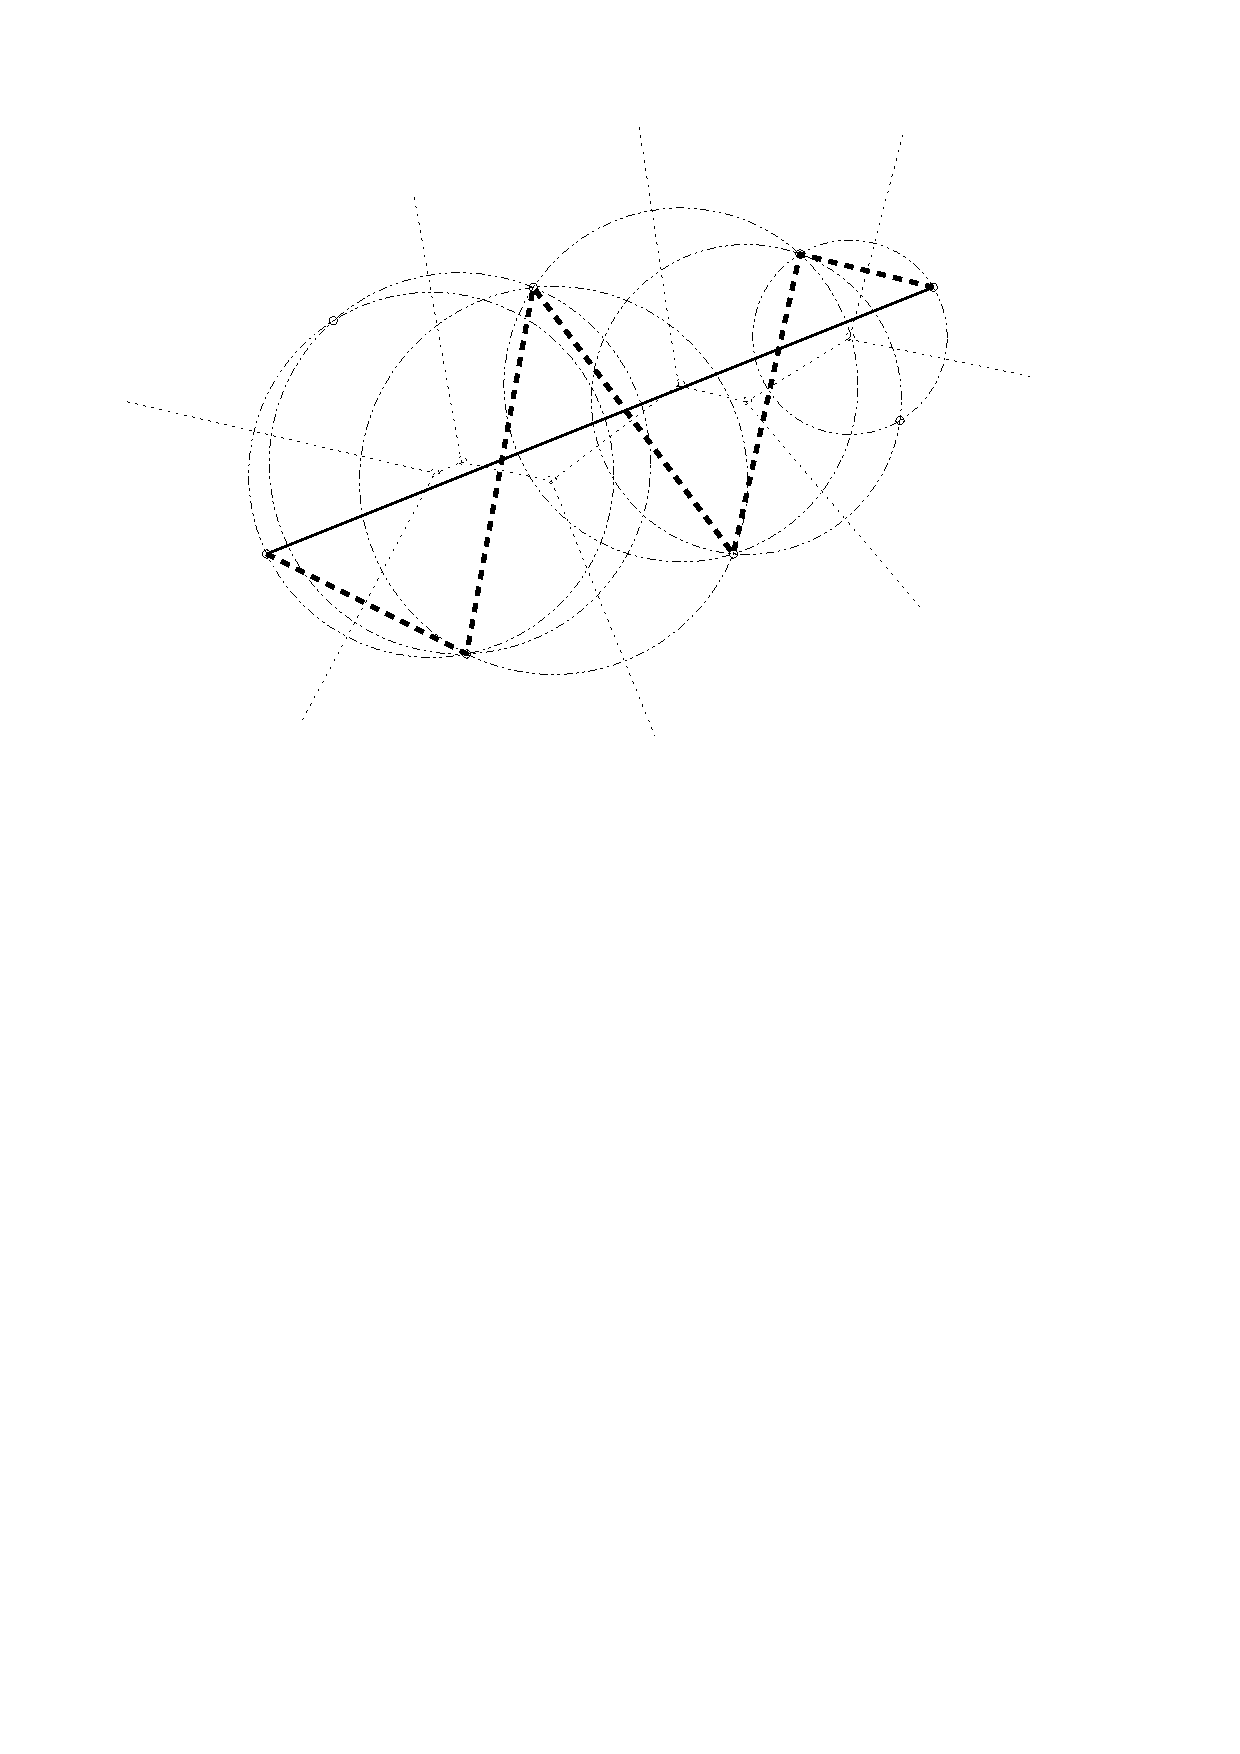
\includegraphics[scale=0.75]{figures/two-sided_path.pdf}

\part{Keil's Results}

TODO

% Content ends here

\newpage

\bibliography{references} % uncomment line to add references

\end{document}
